\hypertarget{aufgabenstellung}{%
\section{Aufgabenstellung}\label{aufgabenstellung}}

Die Idee des Projektes ist es einen Kubernetes Cluster auf 3 VMS zu
deployen und die Möglichkeiten die dadurch entstehen zu erkunden.

Ein optionales Ziel ist es, diese Infrastruktur auf eine Web-Applikation
mit Anbindung einer Datenbank anzuwenden und Aktivitäten zu überprüfen.

\hypertarget{kubernetes}{%
\subsection{Kubernetes}\label{kubernetes}}

Kubernetes ist ein Open-Source Orchestrierungs Tool, das dazu dient
Container automatisiert Bereitzustellen und zu verwalten.

\begin{quote}
Der Name Kubernets kommt aus dem griechischen und steht für Steuermann.
\end{quote}

Wir verwenden in unserem Projekt \href{https://www.docker.com/}{Docker}
als Container Runtime.

\hypertarget{aufbau-und-architektur}{%
\subsubsection{Aufbau und Architektur}\label{aufbau-und-architektur}}

\begin{figure}
\centering
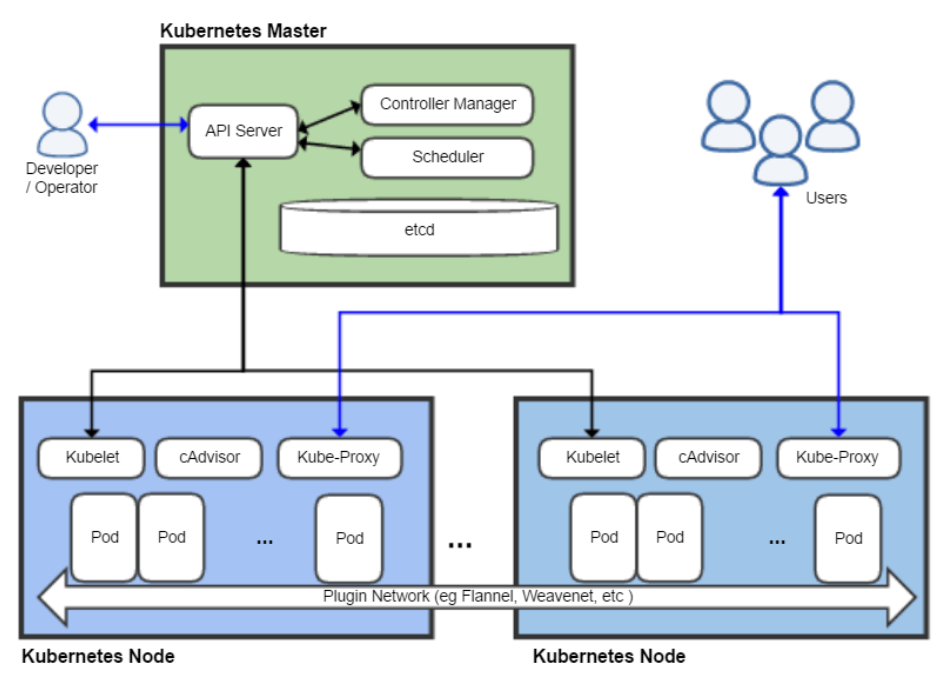
\includegraphics{kuber.png}
\caption{Kubernetes Architektur}
\end{figure}

Der Vorteil bei Kubernetes liegt darin, dass die es \emph{Pods}
orchestriert. Sie stellen die kleinstmögliche Steuerbare Einheit im
Kubernetes Universum dar. Sie laufen auf \emph{Nodes} - also VMs oder
physischen Maschinen). Ein Pod kann einen oder mehrere Container
beinhalten.

Die Architektur ist auf dem Master-Slave System aufgebaut.

Der Master ist die \emph{Control Plane}, auf ihr wird Inventur über alle
Objekte in einem Cluster geführt. Der Master steuert außerdem alle
Slaves (Minions). Wir haben in unserem Fall nur einen Master-Node. Es
können aber auch - zwecks Redundanz - mehre Master-Nodes in einem
Kubernetes Cluster konfiguriert werden.

Auf jedem Minion muss zusätzlich auch die zu verwendente
Container-Runtime installiert werden.

\hypertarget{installation}{%
\section{Installation}\label{installation}}

\hypertarget{validierung-bevor-es-losgeht}{%
\subsection{Validierung bevor es
losgeht}\label{validierung-bevor-es-losgeht}}

Bei jedem Node (VM oder physische Maschine), die im Cluster verwendet
werden soll, müssen sich folgende Eigenschaften unterscheiden:

\begin{longtable}[]{@{}ll@{}}
\toprule
Eigenschaft & Befehl zum Prüfen\tabularnewline
\midrule
\endhead
MAC Adresse & \passthrough{\lstinline!ip link!}\tabularnewline
Produkt UUID &
\passthrough{\lstinline!cat /sys/class/dmi/id product\_uuid!}\tabularnewline
\bottomrule
\end{longtable}

Da wir für dieses Beispiel Debian 10 verwenden, müssen wir zusätzlich
noch iptables in den legacy-mode schalten.

\begin{lstlisting}
update-alternatives --set iptables /usr/sbin/iptables-legacy
update-alternatives --set ip6tables /usr/sbin/ip6tables-legacy
update-alternatives --set arptables /usr/sbin/arptables-legacy
update-alternatives --set ebtables /usr/sbin/ebtables-legacy
\end{lstlisting}

\hypertarget{installation-1}{%
\section{Installation}\label{installation-1}}

\hypertarget{docker}{%
\subsection{Docker}\label{docker}}

Als Container Runtime benutzen wir für dieses Beispiel Docker.

Zuerst müssen wir alle Dependencies von Docker installieren.

\begin{lstlisting}
apt update
apt -y install apt-transport-https ca-certificates curl gnupg2 software-properties-common
\end{lstlisting}

Anschließend fügen für den offiziellen GPG-Key von Docker zu unserem
Package-Manager hinzu. Mit diesem Schlüssel sind die Packete signiert.

\begin{lstlisting}
curl -fsSL https://download.docker.com/linux/debian/gpg | apt-key add -
\end{lstlisting}

Nun können wir die offiziellen Docker-Repositories hinzufügen.

\begin{lstlisting}
add-apt-repository \
   "deb [arch=amd64] https://download.docker.com/linux/debian \
   $(lsb_release -cs) \
   stable"
\end{lstlisting}

Die Installation selbst ist nun ziemlich einfach.

\begin{lstlisting}
apt-get update && apt-get install -y \
  containerd.io=1.2.10-3 \
  docker-ce=5:19.03.4~3-0~debian-$(lsb_release -cs) \
  docker-ce-cli=5:19.03.4~3-0~debian-$(lsb_release -cs)
\end{lstlisting}

Zu guter Letzt passen wir noch die Einstellungen für Docker an.

\begin{lstlisting}
cat > /etc/docker/daemon.json <<EOF
{
  "exec-opts": ["native.cgroupdriver=systemd"],
  "log-driver": "json-file",
  "log-opts": {
    "max-size": "100m"
  },
  "storage-driver": "overlay2"
}
EOF

mkdir -p /etc/systemd/system/docker.service.d
\end{lstlisting}

Einen kleinen Restart brauchen wir noch.

\begin{lstlisting}
systemctl daemon-reload
systemctl restart docker
\end{lstlisting}

Wie jeder gute IT-Admin werden verifizieren wir natürlich noch am Ende
die gelungene Installation.

\begin{lstlisting}
docker version
\end{lstlisting}

Falls hier vernünftige Informationen angezeigt werden und keine
Fehlermeldung ist die Installation gelungen.

\hypertarget{kubernetes-1}{%
\subsection{Kubernetes}\label{kubernetes-1}}

Als nächsten Schritt installieren wir Kubernetes. Oder besser gesagt die
3 Services, aus denen unsere Kubernetes Installation bestehen wird.

\begin{itemize}
\tightlist
\item
  kubeadm
\item
  kubelet
\item
  kubectl
\end{itemize}

Dafür benutzen wir einen ähnlichen Ablauf, wie bei Docker. Der
Einfachheit halber ist nun nicht jeder Schritt kommentiert, sondern ein
fertiges Skript zu sehen.

\begin{lstlisting}
apt-get update && sudo apt-get install -y apt-transport-https curl
curl -s https://packages.cloud.google.com/apt/doc/apt-key.gpg | sudo apt-key add -
cat <<EOF | sudo tee /etc/apt/sources.list.d/kubernetes.list
deb https://apt.kubernetes.io/ kubernetes-xenial main
EOF
apt-get update
apt-get install -y kubelet kubeadm kubectl
apt-mark hold kubelet kubeadm kubectl
\end{lstlisting}

Auch hier folgt natürlich wieder die Verifikation.

\begin{lstlisting}
kubeadm version
kubelet --version
kubectl version
\end{lstlisting}

\hypertarget{erstellung-eines-clusters}{%
\section{Erstellung eines Clusters}\label{erstellung-eines-clusters}}

\hypertarget{einstellungen}{%
\subsection{Einstellungen}\label{einstellungen}}

Ein kleiner Schritt hält uns noch vom Cluster ab: Wir müssen swap
abschalten.

\begin{lstlisting}
swapoff -a
cp /etc/fstab /etc/fstab.orig
cat /etc/fstab.orig | grep -v 'swap' > /etc/fstab
\end{lstlisting}

Jetzt noch ein Reboot.

\begin{lstlisting}
reboot 0
\end{lstlisting}

\hypertarget{kubeadm}{%
\subsection{Kubeadm}\label{kubeadm}}

Bevor man den Cluster installiert muss man sich für ein pod network
add-on entscheiden. Die Auswahl ist da groß, weswegen wir uns
schlichtweg für das beliebteste Add-On entschieden haben: Flannel

Auf unserem Master führen wir nun folgenden Befehl aus:

\begin{lstlisting}
kubeadm init --pod-network-cidr=10.244.0.0/16
\end{lstlisting}

Mit den anderen Nodes können wir jetzt joinen. Den Befehl dafür finden
wir im Output von kubeadm init am Master.

\begin{lstlisting}
kubeadm join 10.0.0.88:6443 --token <token> \
    --discovery-token-ca-cert-hash sha256:<hash>
\end{lstlisting}

\hypertarget{troubleshooting}{%
\section{Troubleshooting}\label{troubleshooting}}

Bei der Verifizierung am Master mit
\passthrough{\lstinline!kubectl get nodes!} kann es zu folgendem Fehler
kommen:

\begin{lstlisting}
The connection to the server localhost:8080 was refused - did you specify the right host or port?
\end{lstlisting}

Das lässt sich mit den folgenden Befehlen beheben. (Credits an den
\href{https://github.com/kubernetes/kubernetes/issues/44665\#issuecomment-295216655}{GitHub
post von user csarora})

\begin{lstlisting}
cp /etc/kubernetes/admin.conf $HOME/
chown $(id -u):$(id -g) $HOME/admin.conf
export KUBECONFIG=$HOME/admin.conf
\end{lstlisting}
